%----------------------------------------------------------------------------------------
%	PACKAGES AND OTHER DOCUMENT CONFIGURATIONS
%----------------------------------------------------------------------------------------

\documentclass[paper=a4, fontsize=11pt]{scrartcl} % A4 paper and 11pt font size

\usepackage[T1]{fontenc} % Use 8-bit encoding that has 256 glyphs
\usepackage{fourier} % Use the Adobe Utopia font for the document - comment this line to return to the LaTeX default
\usepackage[english]{babel} % English language/hyphenation
\usepackage{amsmath,amsfonts,amsthm} % Math packages

\usepackage{lipsum} % Used for inserting dummy 'Lorem ipsum' text into the template

\usepackage{sectsty} % Allows customizing section commands
\allsectionsfont{\centering \normalfont\scshape} % Make all sections centered, the default font and small caps
\usepackage{graphicx}
\usepackage{fancyhdr} % Custom headers and footers
\pagestyle{fancyplain} % Makes all pages in the document conform to the custom headers and footers
\fancyhead{} % No page header - if you want one, create it in the same way as the footers below
\fancyfoot[L]{} % Empty left footer
\fancyfoot[C]{} % Empty center footer
\fancyfoot[R]{\thepage} % Page numbering for right footer
\renewcommand{\headrulewidth}{0pt} % Remove header underlines
\renewcommand{\footrulewidth}{0pt} % Remove footer underlines
\setlength{\headheight}{13.6pt} % Customize the height of the header

\numberwithin{equation}{section} 
\numberwithin{figure}{section} 
\numberwithin{table}{section} 

\setlength\parindent{0pt} 

%----------------------------------------------------------------------------------------
%	TITLE SECTION
%----------------------------------------------------------------------------------------

\newcommand{\horrule}[1]{\rule{\linewidth}{#1}}

\title{	
\normalfont \normalsize 
\textsc{Harvard University} \\[25pt]
\textsc{CS281} \\[25pt]
\horrule{0.5pt} \\[0.4cm] 
\huge Final Project Update: \\
\huge Classification for the Yelp Data Set Challenge
\horrule{2pt} \\[0.5cm]
}

\author{Nicolas Drizard \& Virgile Audi}

\date{\normalsize\today} 
\begin{document}

\maketitle

\section{Abstract Draft}

\section{Numerical processing and first clustering experiments}

\section{Text preprocessing and LDA}
\subsection{Text preprocessing}
An important part of these first days of work was processing the text reviews on which we would perform LDA. The reviews came in the form of json file with information such as:
\begin{itemize}
\item the business id of the business reviewed,
\item the reviewer's id,
\item the number of stars given
\item the text of the review itself in the form of a string
\item and some extra information such as the class of review (fun,useful and others) based on Yelp users' votes.
\end{itemize}

We were first interested in extracting the business ids and the text reviews. The length of the texts varied a lot. Inspecting the data, we can find reviews of a line only and reviews much longer. Our motivation for this project is to classify the venues based on the text reviews, so the identity of the reviewers does not matter. We therefore merged the reviews by venues. We reduced the 1.6 million reviews to a corpus of 60785 larger texts, 1 per business. Note that we first had to clean the texts by removing capital letters, digits, etc... \\

As LDA uses the bag-of-words assumption, we only wanted to keep words that had a semantic interest. So we removed a list of stop words based on the most common words in the English language such as: "is, a, I, 'm, 's, and, can, be, etc...". This yield a total vocabulary of over 400 thousands unique words, which dazzled us at first, but we'll come back on that issue later. We then transformed the corpus into a sparse matrix for which each row corresponds to a document and column $j$ tracks the count of the word indexed by $j$ in the vocabulary. This step made our computers' ipython kernel crash multiple time but we finally obtained a sparse matrix of size 140 GB.\\

The size of the document-term frequency (dtf) matrix being too big to work with, we decided to focus only on restaurant type of businesses (the yelp data set contains reviews about dentists, supermarkets, etc.). Reprocessing everything yielded a corpus of about 18000 venues, and a total vocabulary of 200 000 words. Reevaluating the dtf matrix was then much easier. We then persued to fit a baseline LDA model using the lda 1.0.2 python package. But the computation ended up being way to expensive timewise (we left the algorithm run for 8 hours and still didn't converge even though we enforced a maximum number of iterations of 1500!). In order to show some results for this update, we subsambled 500 restaurants and ran the algorithm again. Subsampling had for consequence to reduce the size of the vocabulary to only $\sim$40 000 words. Completion time for the algorithm was about an hour for 50 topics. Some of the results are shown below:

\begin{figure}[h!]
\centering
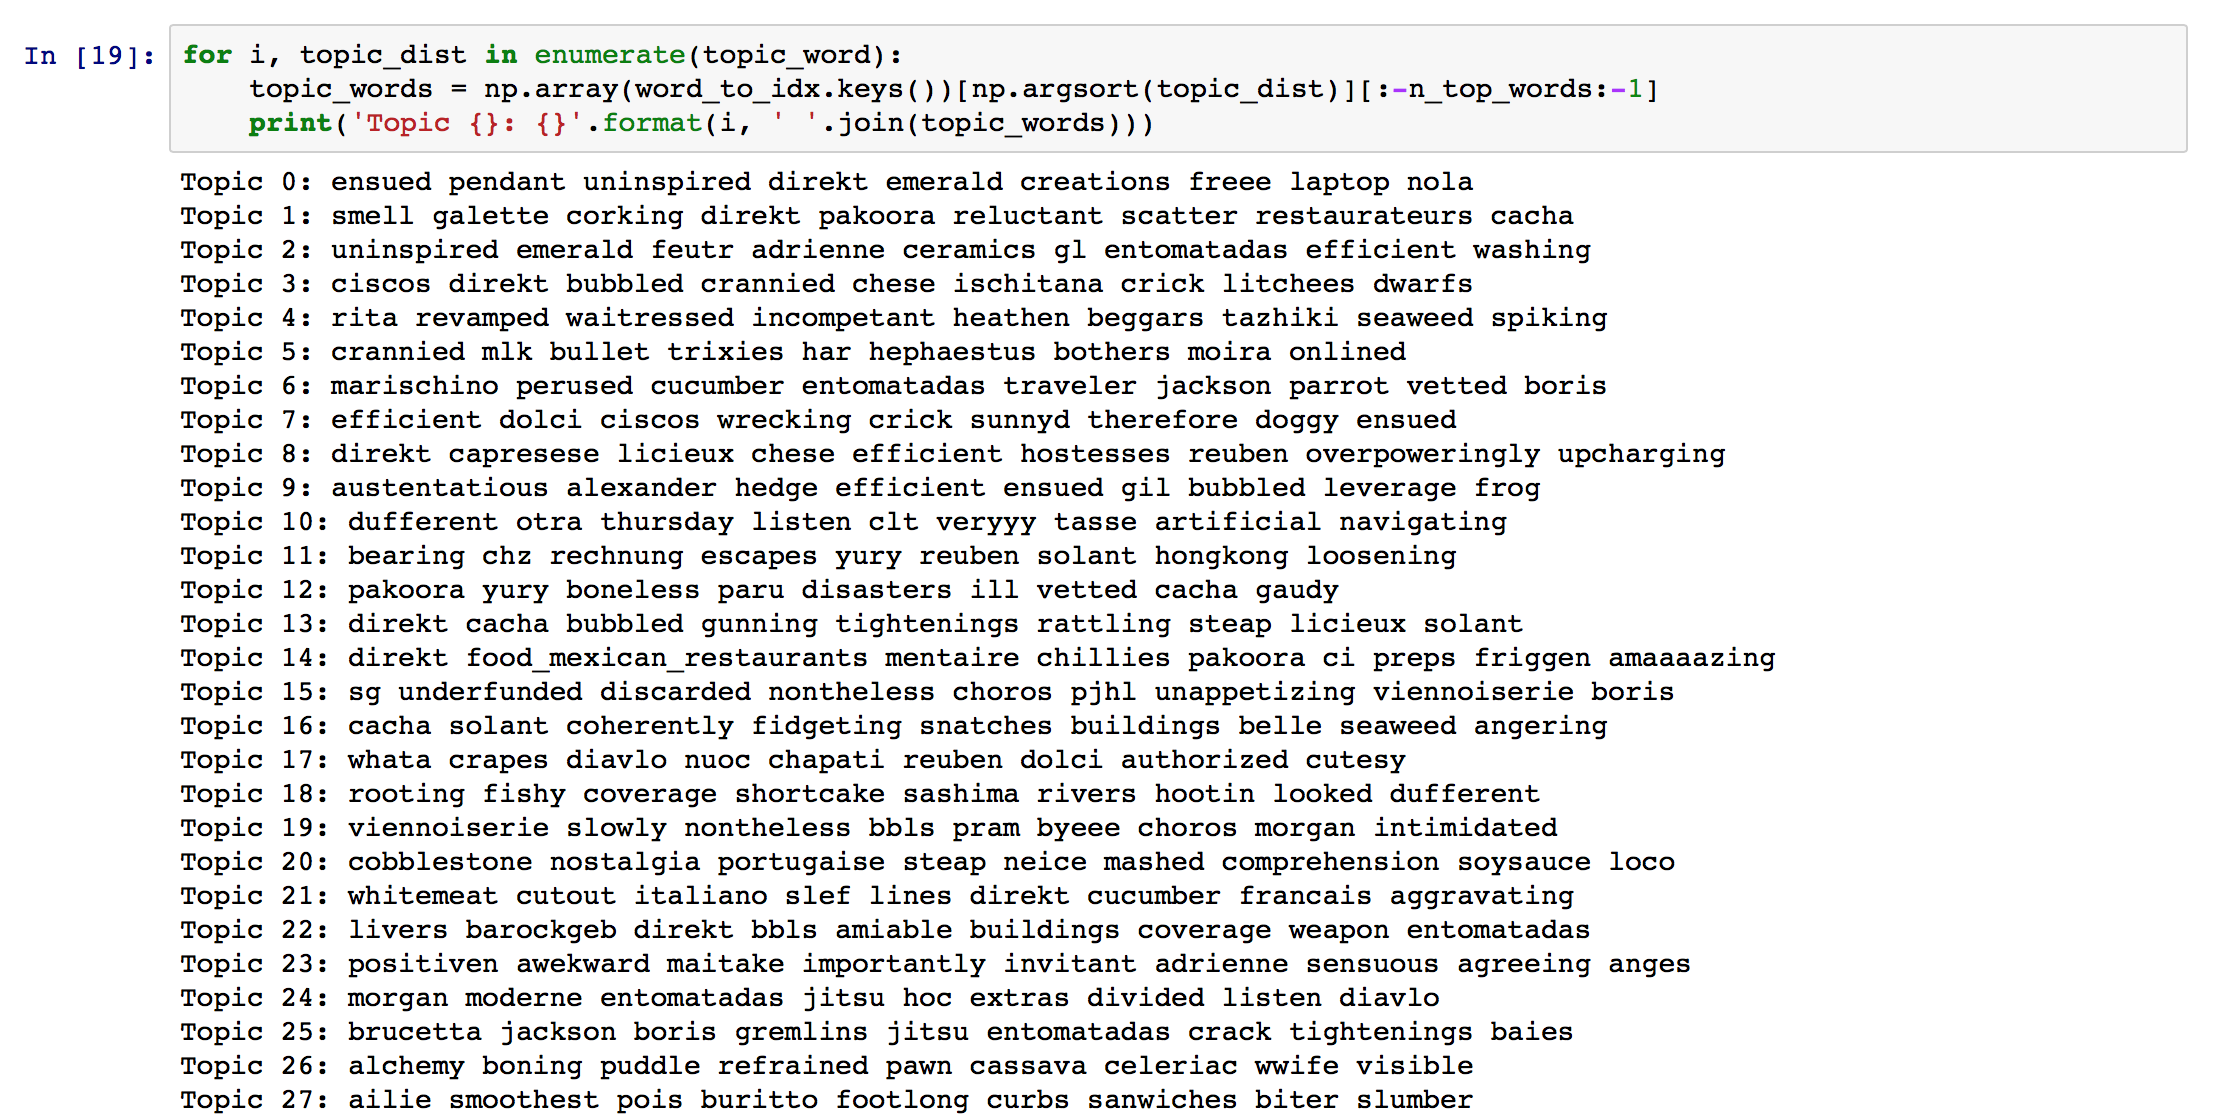
\includegraphics[width=1\textwidth]{first_topics.png}
\end{figure}

The topics obtained a very poor and there are numerous reasons for that. The first is that we didn't get the chance to cross-validate the number of topics queried. The second is that we then noticed that we had an issue, that might result to be very problematic, with spelling. If any of the TFs have suggestions on how to tackle this issue, we would greatly appreciate it. A third reason might lie in the fact that we are failing to distinguish what constitutes the reviewer's opinion (is it good restaurant? is it bad?) and what is this restaurant about (Italian? Japanese?). This third reason motivated the analysis of a customed LDA model that we will describe below. We haven't yet done any type of analysis but this is the model that we will now focus on and code up. This will alow us to use the regular LDA as a baseline to compare new topics.\\

\subsection{The custom LDA model}

The assumption that we will make for this model is the following: each review can be divided into two parts,
\begin{itemize}
\item words coming from an opinion topic that correspond to the rating of the review (in this particular case, we will use 5 topics for 5 stars),
\item and words coming from any type of content topics.
\end{itemize}
For simplicity reason, we will also assume that the proportion of words from each part is fixed, for instance 30:70 or 40:60. Depending on the performance of this new method, we might decide to relax this last assumption and try to learn this parameter as well.\\

The new generative process for each review $r$ will therefore be:
\begin{enumerate}
\item Generate the length using a Poisson distribution: $N_r \sim \text{Poisson}(\xi)$
\item Choose an opinion topic: $o_r \sim \text{Cat}(\beta)$, where $\beta \in \mathbb{R}^5$ 
\item Draw the per-document content topic distribution: $c_r\sim \text{Dir}(\alpha)$
\item For each word $w_{ri}$,\quad generate $u \sim \text{Unif}(0,1)$:
	\begin{enumerate}
	\item If $u<=p$ where p is the fixed proportion ruling the opinion/content separation then:
		\begin{itemize}
		\item Pick a word $p(w_{ri} | o_r) \sim \text{Cat}(o_r)$
		\end{itemize}
	\item If $u>p$ then:
		\begin{itemize}
		\item Choose a latent content topic: $z_i \sim \text{Cat}(c_r)$
		\item Choose a word $p(w_{ri} | z_n) \sim \text{Cat}(z_n)$
		\end{itemize}
	\end{enumerate}
\end{enumerate}
The mathematics behind shouldn't be too different from the derivations in the regular LDA model. We shall investigate this new model in the next few days.
\end{document}